\documentclass[a4paper,12pt]{article} %размер бумаги устанавливаем А4, шрифт 12пунктов
\usepackage[utf8]{inputenc}
\usepackage{csquotes}
\usepackage[english,russian]{babel}%используем русский и английский языки с переносами
\usepackage{biblatex}
\bibliography{refs}
\usepackage{amssymb,amsfonts,mathtext,enumerate,float} %подключаем нужные пакеты расширений
\usepackage{textcomp}
\usepackage{adjustbox}
\usepackage{graphicx} %хотим вставлять в диплом рисунки?
\makeatletter
\makeatother
\usepackage{sagetex}
\usepackage{geometry} % Меняем поля страницы
\geometry{left=2cm}% левое поле
\geometry{right=1.5cm}% правое поле
\geometry{top=1cm}% верхнее поле
\geometry{bottom=2cm}% нижнее поле
\usepackage{tabularx}
\usepackage{threeparttable}
\usepackage{epstopdf}
\usepackage{amsmath} %отображение математической нотации
\usepackage{caption, subcaption} %подписи}
\usepackage{indentfirst}%отступ вначале параграфа
\usepackage{pscyr}
%\usepackage{natbib}
%\usepackage{ragged2e} %для таблиц

\captionsetup[table]{labelsep = endash, singlelinecheck=false}
\captionsetup[figure]{name = Рисунок, labelformat=simple, labelsep = endash}


\begin{document}


\newcommand\tline[2]{$\underset{\text{#1}}{\text{\underline{\hspace{#2}}}}$}
\newcommand\nameLine[3]{$\underset{\text{#1}}{\text{\underline{\text{#2}\hspace{#3}}}}$}

\begin{titlepage}
	\centering
	{\fontsize{12pt}{5cm}\selectfont \bfseries Министерство образования и науки Российской Федерации} \\ \vspace{0.5cm}
	{\fontsize{7pt}{5cm}\selectfont ФЕДЕРАЛЬНОЕ ГОСУДАРСТВЕННОЕ АВТОНОМНОЕ ОБРАЗОВАТЕЛЬНОЕ УЧРЕЖДЕНИЕ ВЫСШЕГО ПРОФЕССИОНАЛЬНОГО ОБРАЗОВАНИЯ} \\ 
	\vspace{1cm}
	{\fontsize{12pt}{5cm}\selectfont \bfseries САНКТ-ПЕТЕРБУРГСКИЙ УНИВЕРСИТЕТ ИНФОРМАЦИОННЫХ ТЕХНОЛОГИЙ, МЕХАНИКИ И ОПТИКИ} \\ \vspace{1.5cm}
	
	{\fontsize{14pt}{5cm}\selectfont Кафедра \hspace{1cm} \underline{Систем Управления и Информатики}  \hspace{1cm} Группа \underline{Р3340}} \\
	
	\vspace{2cm}
	
	{\fontsize{20pt}{5cm}\selectfont \bfseries Лабораторная работа №9} \\
	{\fontsize{20pt}{5cm}\selectfont \bfseries “Экспериментальное построение частотных характеристик типовых динамических звеньев”} \\
	\vspace{0.2cm}
	{\fontsize{14pt}{5cm}\selectfont Вариант - 10} \\
	
	\vspace{1.5cm}
	
	\flushleft
	{Выполнилa \hspace{1.8cm} \nameLine{(фамилия, и.о.)}{Ким А. А.}{7cm} (подпись)} \\
	
	\vspace{2cm}
	
	{Проверил \hspace{2cm} \tline{(фамилия, и.о.)}{9cm} (подпись)} \\
	
	\vspace{5cm}
	
	"\underline{\hspace{0.7cm}}"\hspace{0.2cm}\underline{\hspace{2cm}}\hspace{0.2cm}20\underline{\hspace{0.7cm}}г. \hspace{2cm} Санкт-Петербург, \hspace{2cm} 20\underline{\hspace{0.7cm}}г. \\ \vspace{1cm}
	
	Работа выполнена с оценкой \hspace{1cm} \underline{\hspace{8cm}} \\ 
	\vspace{1cm}
	Дата защиты "\underline{\hspace{0.7cm}}"\hspace{0.2cm}\underline{\hspace{2cm}}\hspace{0.2cm}20\underline{\hspace{0.7cm}}г.
\end{titlepage}
\setcounter{page}{2}

\paragraph{Цель работы:}Изучение математических моделей и исследование характеристик электромеханического объекта управления, построенного на основе электродвигателя постоянного тока независимого возбуждения.
\paragraph{Исходные данные.}
Функциональная схема типичного электромеханического объекта (ЭМО) представлена на рисунке \ref{EMO}. Она включает усилительно-преобразовательное устройство (УПУ), электродвигатель (ЭД), редуктор (Р) и исполнительный механизм (ИМ). \par
Усилительно-преобразовательное устройство служит для формирования напряжения, подаваемого на двигатель в соответствии с управляющим сигналом. Электродвигатель осуществляет преобразование электрической энергии в механическую. Редуктор снижает скорость вращения и повышает момент двигателя на валу ИМ. Для получения информации о состоянии объекта, используемой в устройстве управления, ЭМО снабжено измерительным устройством углового или линейного перемещения (измерители перемещения — ИП).
\begin{figure}[h!]
    \centering
    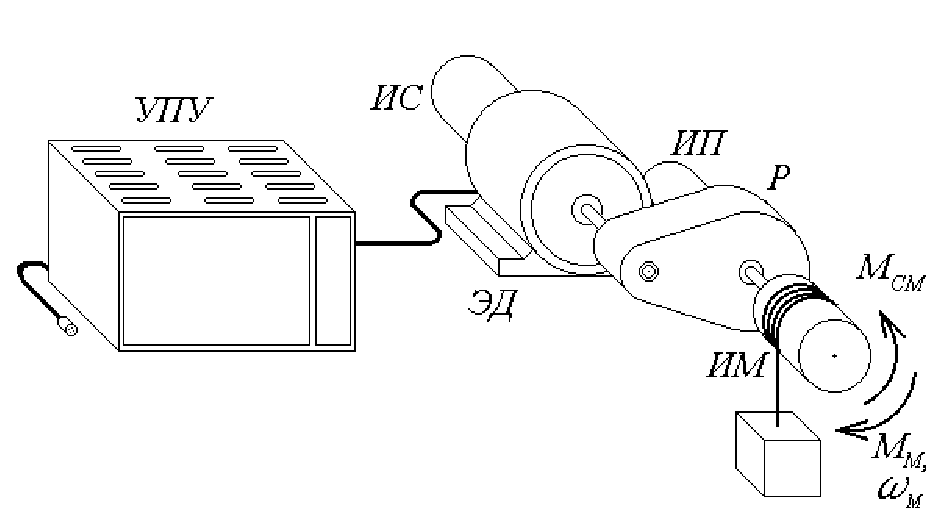
\includegraphics[width = 0.9\textwidth]{scheme/EMO}
    \caption{Функциональная схема ЭМО}
    \label{EMO}
\end{figure}

Исходные данные для выполнения работы приведены в таблице \ref{Tab1}.
\begin{table}[h!]
	\renewcommand{\arraystretch}{1.3} %строки
	\renewcommand{\tabcolsep}{0.3cm} %столбцы
	\centering
	\begin{threeparttable}
	    \caption{Исходные данные}
	    \begin{tabular}{|c|c|c|c|c|c|c|c|c|c|}
		    \hline $U_H,$ & $n_0,$ & $I_H,$ & $M_H,$ & R, & $T_\text{Я},$ & $J_\text{Д},$ & $T_\text{У},$ & $i_p$ & $J_M,$\\
		    В & \text{об/мин} & А & Н$\cdot$м & Ом & мc & кг$\cdot$м$^2$ & мс &  & кг$\cdot$м$^2$\\
		    \hline 65 &	2000 & 14,7 & 4,6 & 0.65 & 10 & $3,4\cdot10^{-3}$ &	8 &	20 & 2,25\\
		    \hline
	    \end{tabular} 
	    \label{Tab1}
    \end{threeparttable}
\end{table}

\newpage
\section{Расчёт параметров математической модели двигателя}

Произведём расчет необходимых параметров для полной модели:
\begin{gather}
    J_p = 0,2J_\text{Д} = 0,2 \cdot 3,4\cdot10^{-3} = 0,68\cdot10^{-3} [\text{кг}\cdot\text{м}^2]\\
    J_\Sigma = J_\text{Д} + J_p + \frac{J_M}{i_p^2} = 3,4\cdot10^{-3} + 0,68\cdot10^{-3} + \frac{2,25}{20^2} = 0,0097 [\text{кг}\cdot\text{м}^2]\\
    K_E = \frac{U_H}{\omega_0} = \frac{U_H\cdot60}{2\pi\cdot n_0} = \frac{65\cdot60}{2\pi\cdot2000} = 0,31 [B\cdot c/\text{рад}]\\
    K_m = \frac{M_H}{I_H} = \frac{4,6}{14,7} = 0,31 [H\cdot\text{м}/A]\\
    K_\text{Д} = \frac{1}{R} = \frac{1}{0,65} = 1,53 [\text{См}]\\
    K_\text{У} = \frac{U_H}{U_m} = \frac{65}{10} = 6,5 [B]
\end{gather}
\par
Для упрощенной модели:
\begin{gather}
	K = \frac{K_\text{У}}{K_E\cdot i_p} = \frac{6,5}{0,31 \cdot 20} = 1.04 [\text{рад}/c]\\
	K_f = \frac{R}{K_m\cdot K_E\cdot i_p^2} = \frac{0,65}{0,31\cdot0,31\cdot20^2} = 0,016909 [\text{Ом$\cdot$А$\cdot$рад}/(H\cdot\text{м}\cdot B\cdot c)]\\
	T_M = \frac{R\cdot J_\Sigma}{K_m\cdot K_E} = \frac{0,65\cdot0,0097}{0,31\cdot0,31} = 0,065608[\text{Ом$\cdot$А$\cdot$рад$\cdot$кг$\cdot$м$^2$}/(H\cdot B \cdot c)]
\end{gather}
\par
Коэффициенты передачи измерительных устройств $K_U, K_I, K_\omega, K_\alpha$ выбираются таким образом, чтобы обеспечить соответствие максимального значения измеряемого сигнала уровню 10 В на выходе измерительного устройства.\\ 
$K_U = 0,307$\\
$K_I = 0,269$\\
$K_\omega = 0,095$\\
$K_\alpha = 5.847$


\newpage
\section{Математическое моделирование полной модели электромеханического объекта}	 
На основе структурной схемы, представленной на рисунке \ref{scheme/fullScheme}, составим схему моделирования ЭМО (рисунок \ref{scheme1}).
\begin{figure}[ht!]
	\centering
	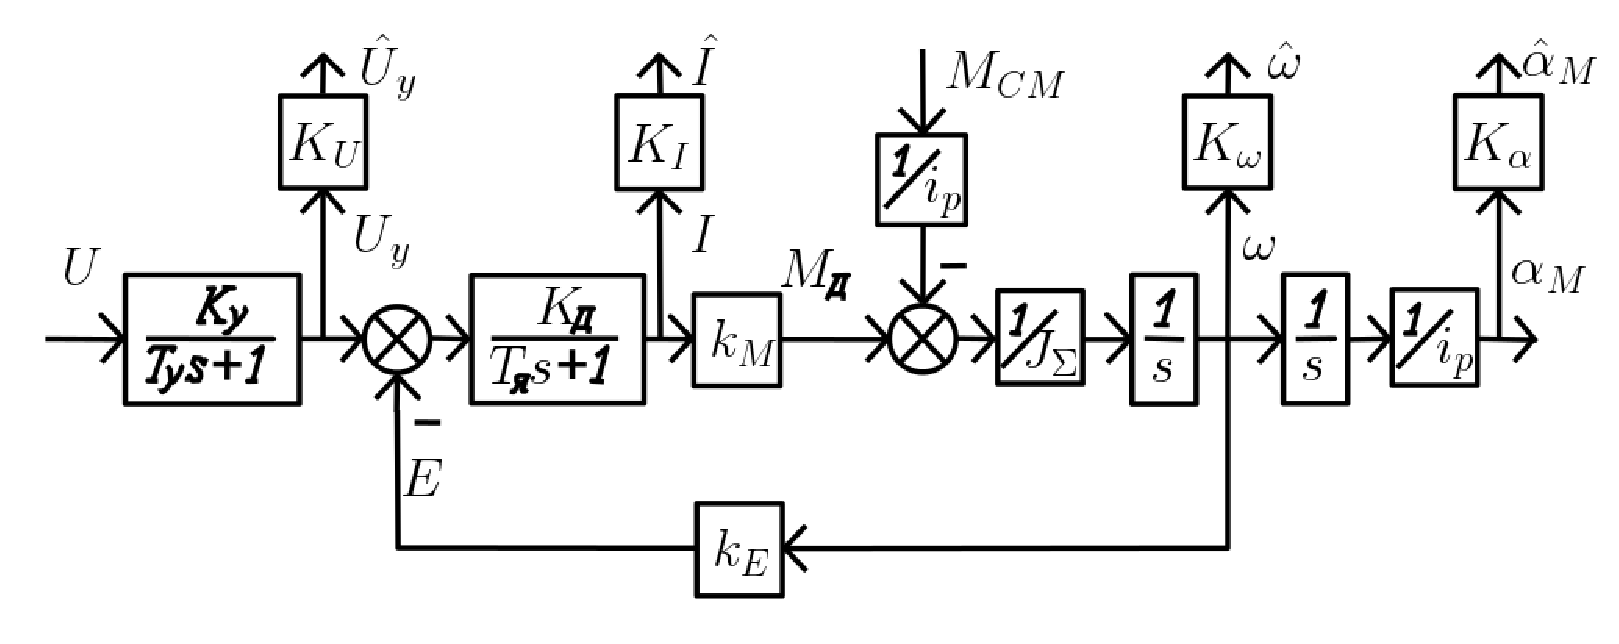
\includegraphics[width = \textwidth]{scheme/fullScheme}
	\caption{Структурная схема ЭМО}
	\label{fullScheme}
\end{figure}
\begin{figure}[ht!]
	\centering
	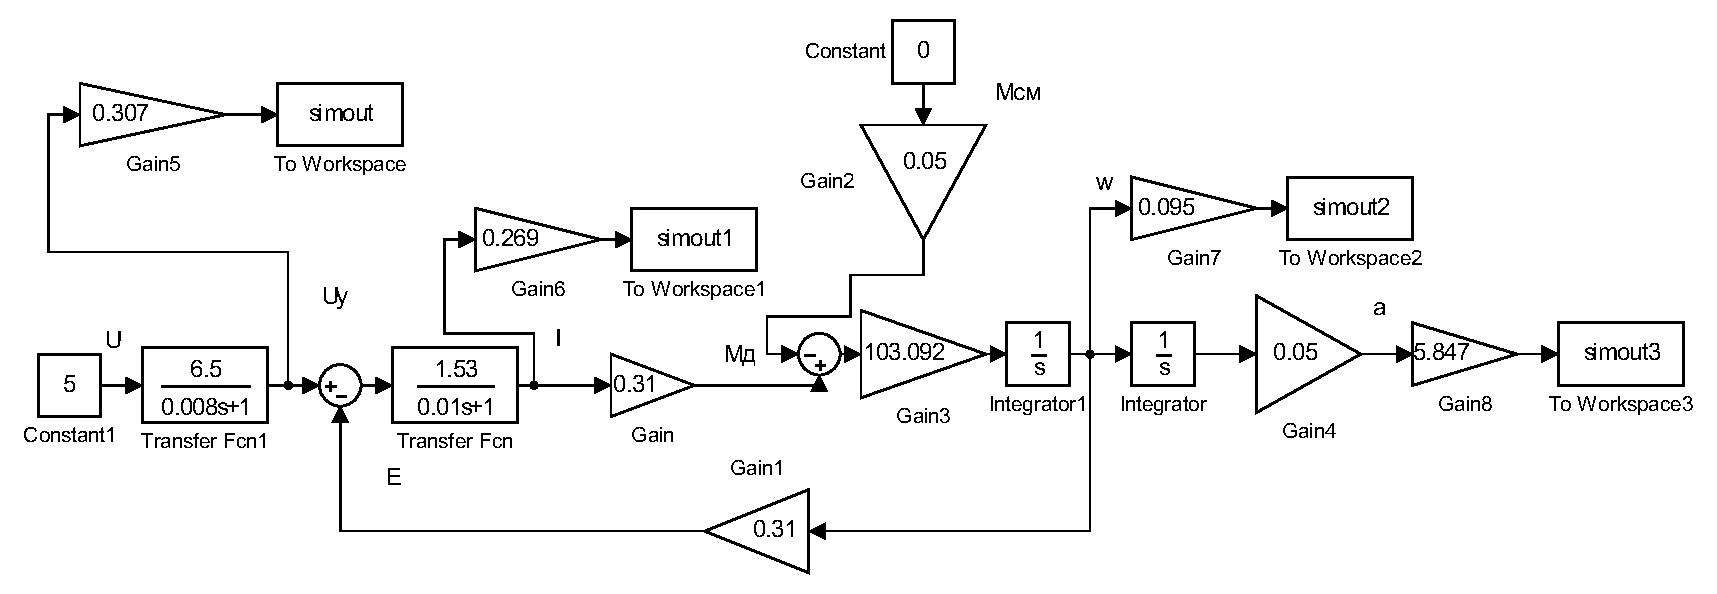
\includegraphics[width = \textwidth]{scheme/scheme1}
	\caption{Схема моделирования ЭМО}
	\label{cxema1}
\end{figure}
\par
Построим графики переходных процессов при $M_{CM}=0$ Н$\cdot$м и U=5B (рисунок \ref{UIwa0}):
\begin{figure}[H]
	\centering
	\begin{subfigure}[b]{0.48\textwidth}
	    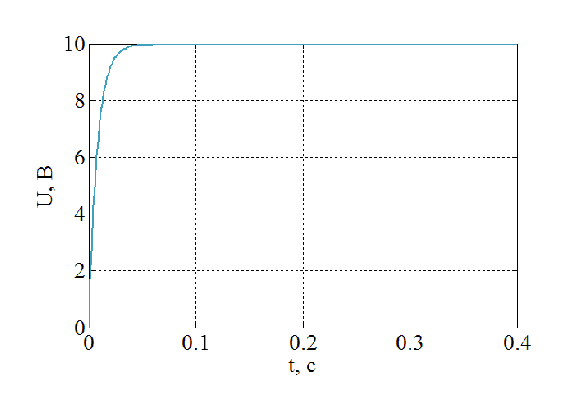
\includegraphics[width = \textwidth]{scheme/U0}
		\caption{Переходный процесс по напряжению}
	\end{subfigure}
	\hfill
	\begin{subfigure}[b]{0.48\textwidth}
		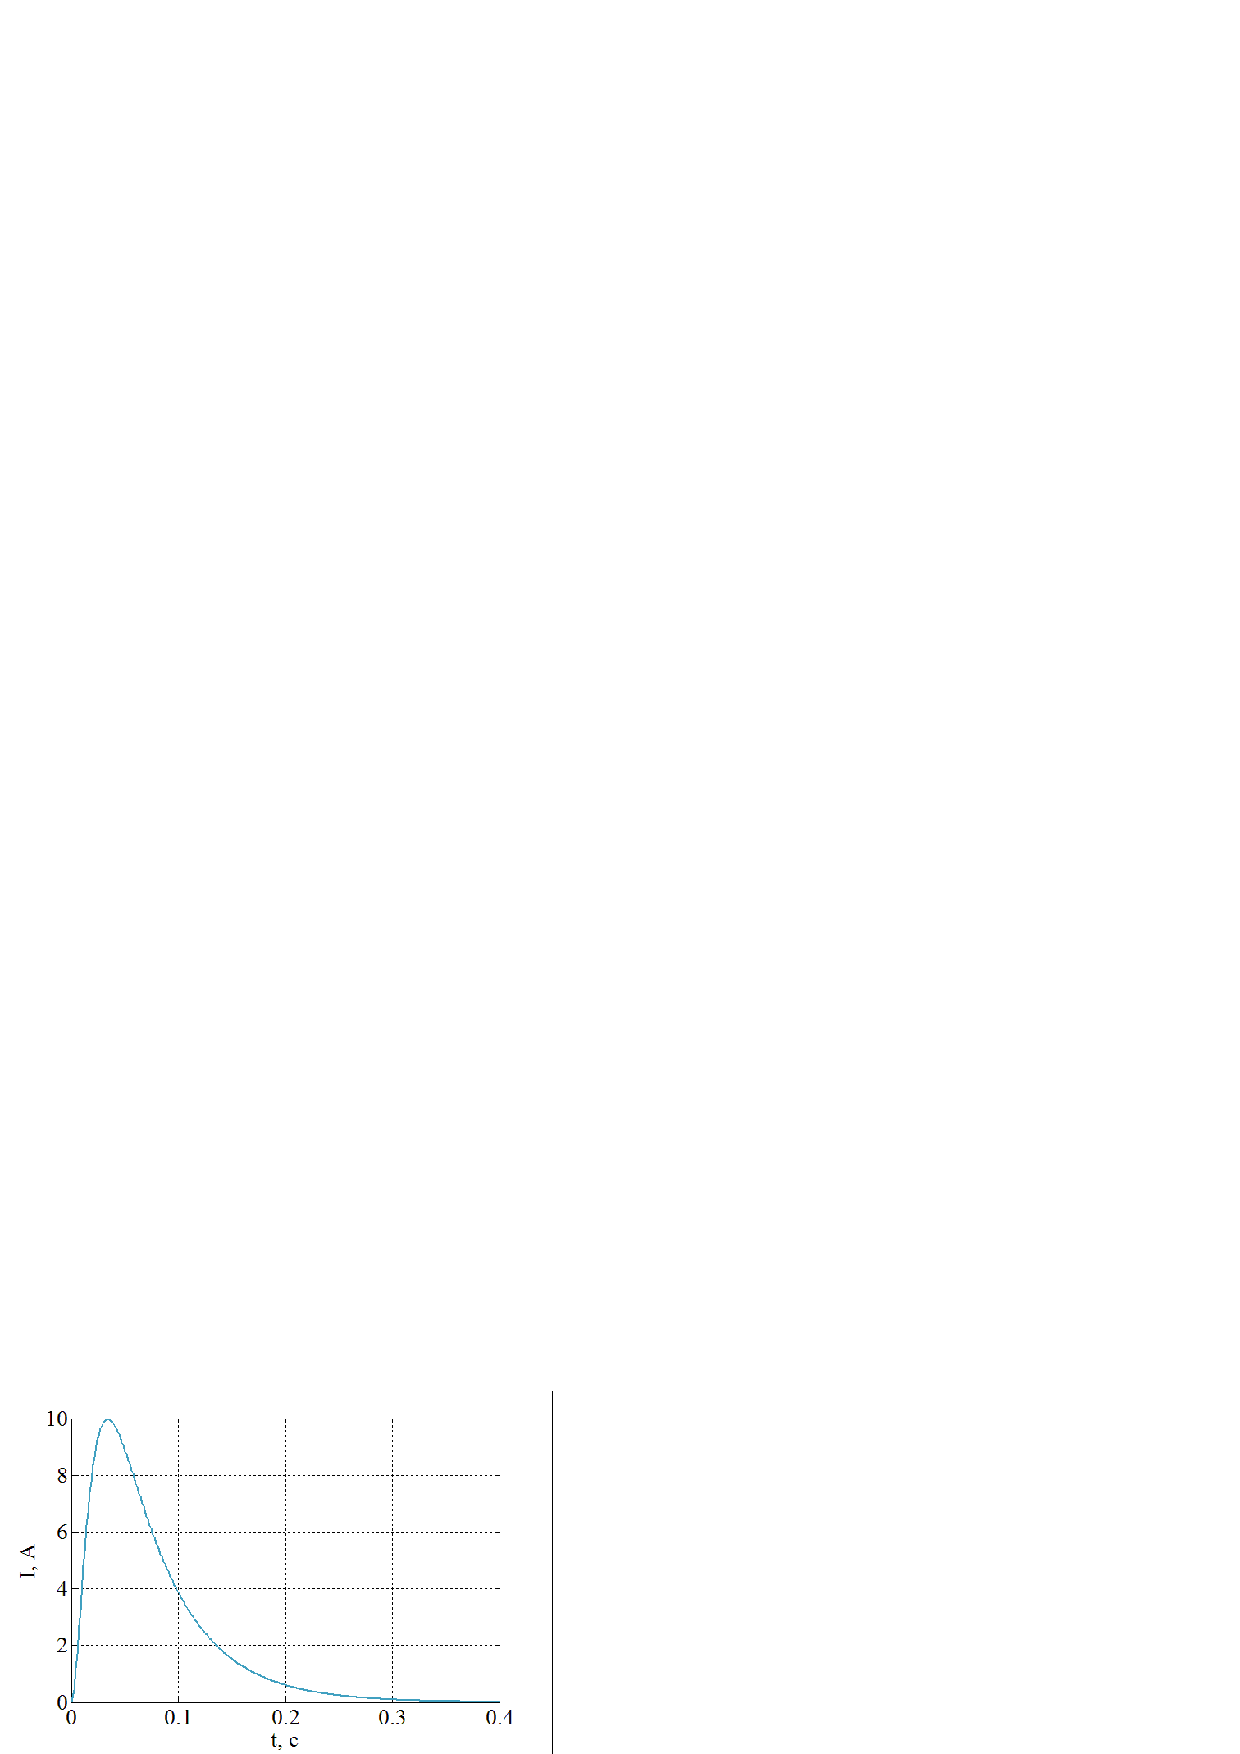
\includegraphics[width = \textwidth]{scheme/I0}
		\caption{Переходный процесс по току}
	\end{subfigure}
	\begin{subfigure}[b]{0.48\textwidth}
		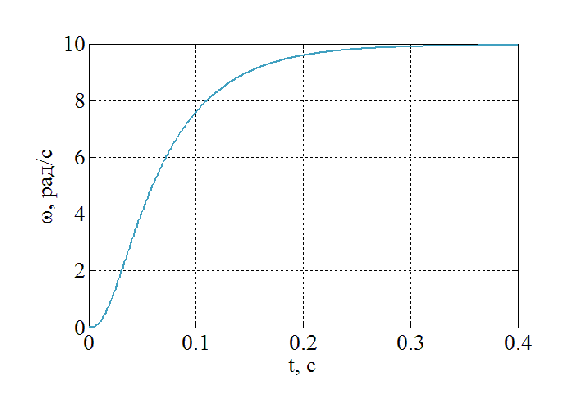
\includegraphics[width = \textwidth]{scheme/W0}
		\caption{Переходный процесс по угловой скорости}
	\end{subfigure}
	\hfill
	\begin{subfigure}[b]{0.48\textwidth}
		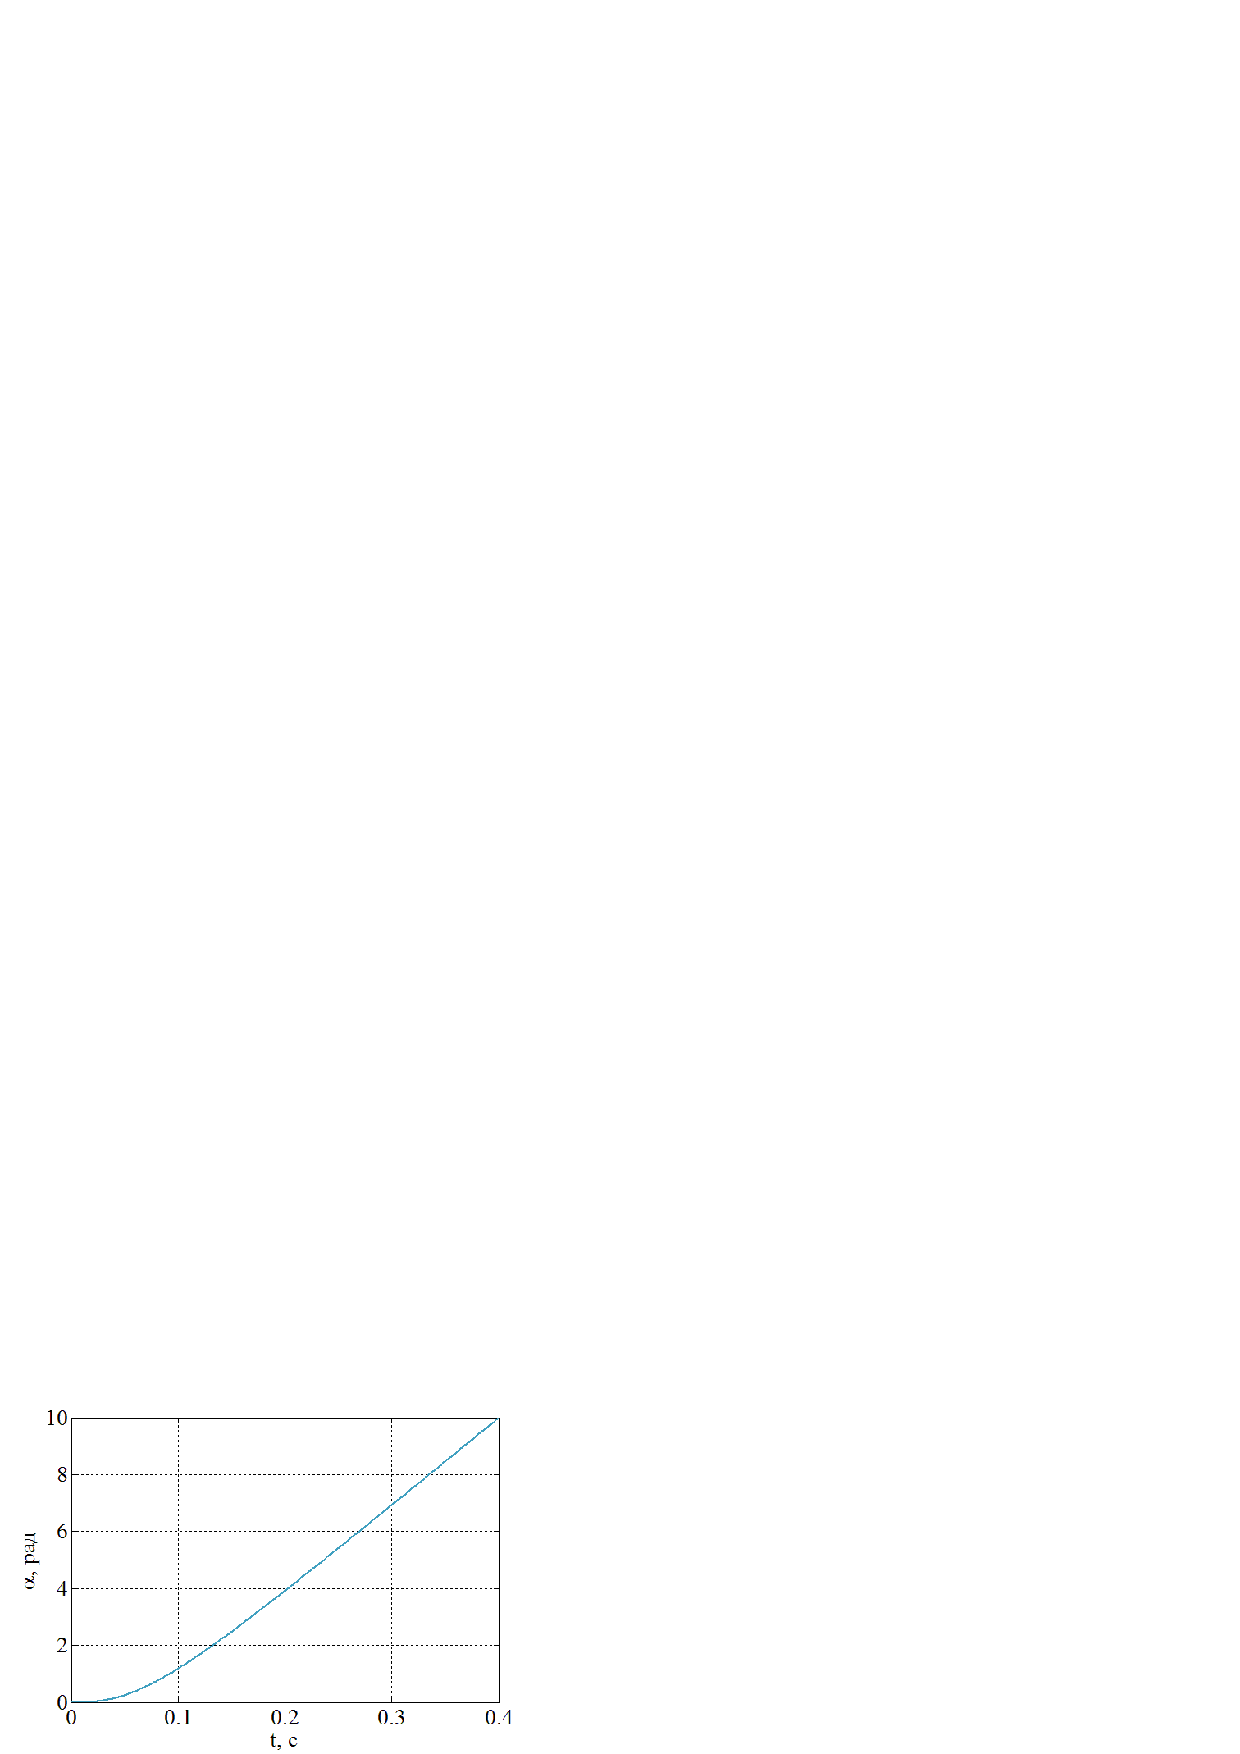
\includegraphics[width = \textwidth]{scheme/A0}
		\caption{Переходный процесс по углу поворота}
	\end{subfigure}
	\caption{Графики переходных процессов при $M_{CM}=0$ Н$\cdot$м и U=5B}
	\label{UIwa0}
\end{figure}

\newpage
\section{Исследование влияния момента сопротивления $M_{CM}$ на вид переходных процессов}
Диапазон изменения $M_{CM}$: от 0 Н$\cdot$м до величины, равной $i_pM_H=92$. Графики переходных процессов представлены на рисунке \ref{UIwa1}.
\begin{figure}[H]
	\centering
	\begin{subfigure}[b]{0.48\textwidth}
	    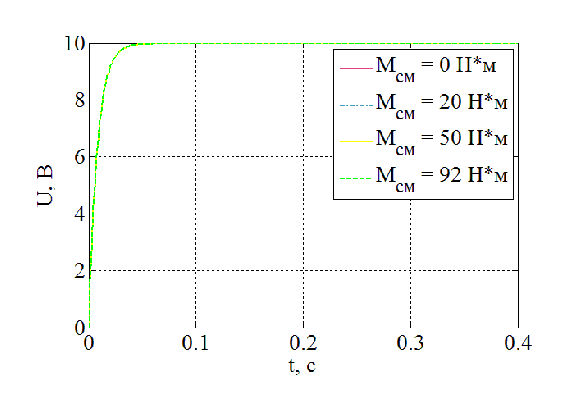
\includegraphics[width = \textwidth]{scheme/U1}
		\caption{Переходный процесс по напряжению}
	\end{subfigure}
	\hfill
	\begin{subfigure}[b]{0.48\textwidth}
		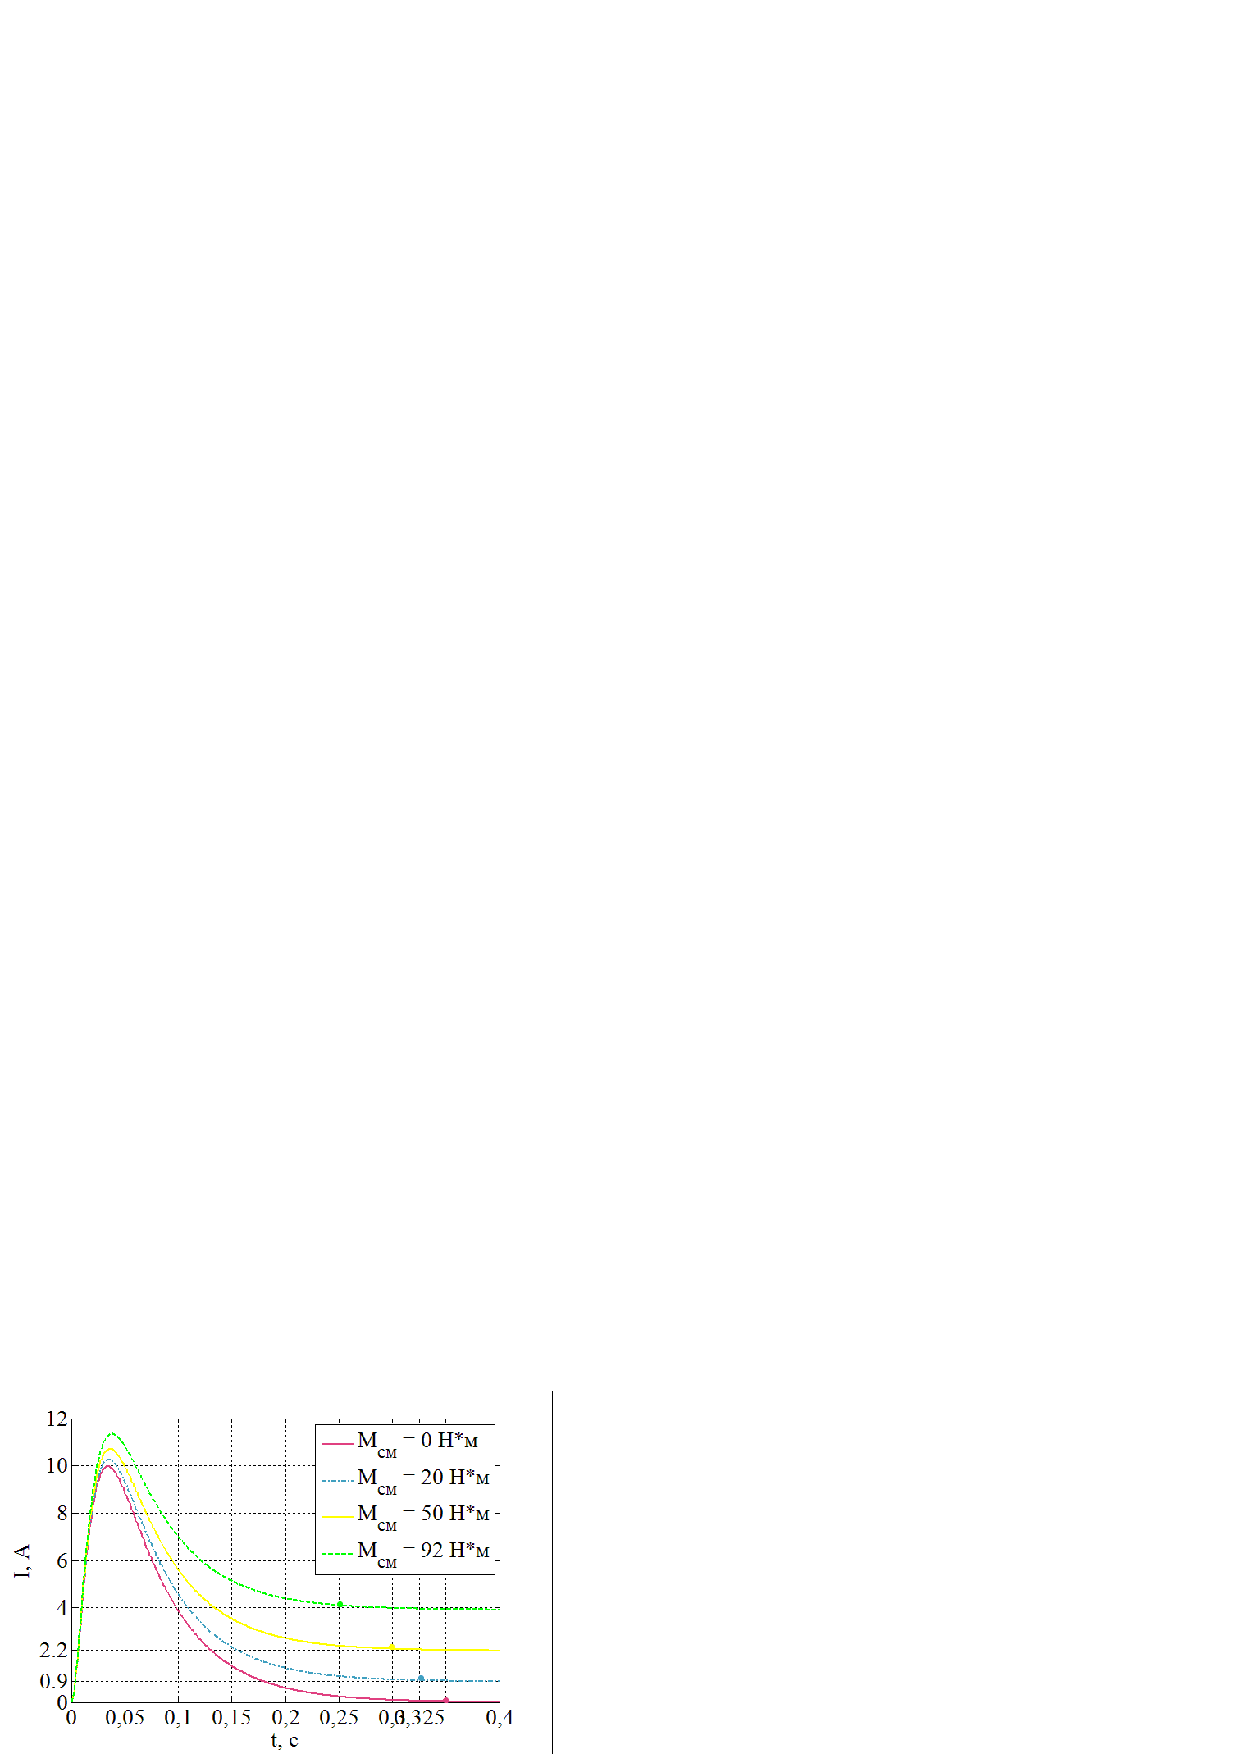
\includegraphics[width = \textwidth]{scheme/I1}
		\caption{Переходный процесс по току}
	\end{subfigure}
	\begin{subfigure}[b]{0.48\textwidth}
		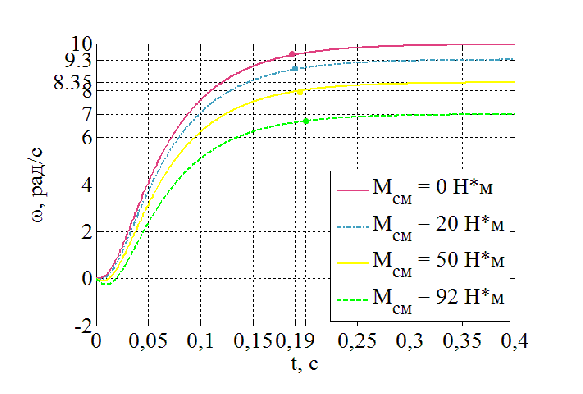
\includegraphics[width = \textwidth]{scheme/W1}
		\caption{Переходный процесс по угловой скорости}
	\end{subfigure}
	\hfill
	\begin{subfigure}[b]{0.48\textwidth}
		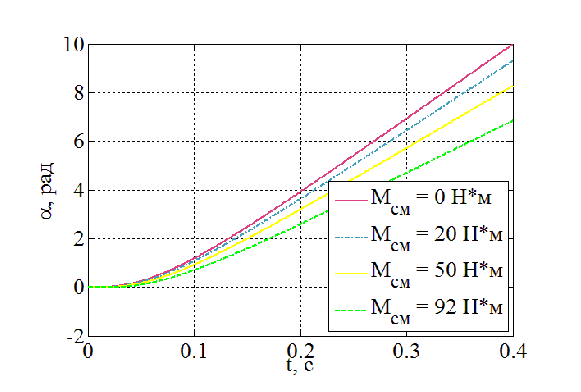
\includegraphics[width = \textwidth]{scheme/A1}
		\caption{Переходный процесс по углу поворота}
	\end{subfigure}
	\caption{Графики переходных процессов при различных значениях $M_{CM}$}
	\label{UIwa1}
\end{figure}

\newpage
\section{Исследование влияния момента нагрузки $J_M$ на вид переходных процессов}
Диапазон изменения момента инерции: $\pm 50\%$  от заданного значения. Графики переходных процессов представлены на рисунке \ref{UIwa2}.
\begin{figure}[H]
	\centering
	\begin{subfigure}[b]{0.48\textwidth}
	    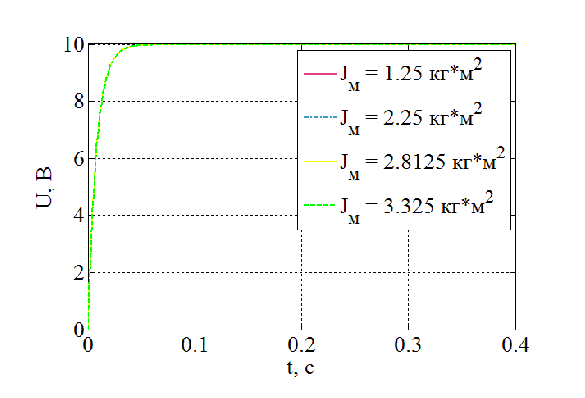
\includegraphics[width = \textwidth]{scheme/U2}
		\caption{Переходный процесс по напряжению}
	\end{subfigure}
	\hfill
	\begin{subfigure}[b]{0.48\textwidth}
		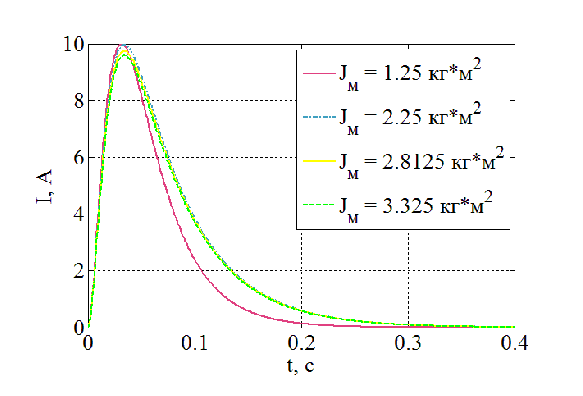
\includegraphics[width = \textwidth]{scheme/I2}
		\caption{Переходный процесс по току}
	\end{subfigure}
	\begin{subfigure}[b]{0.48\textwidth}
		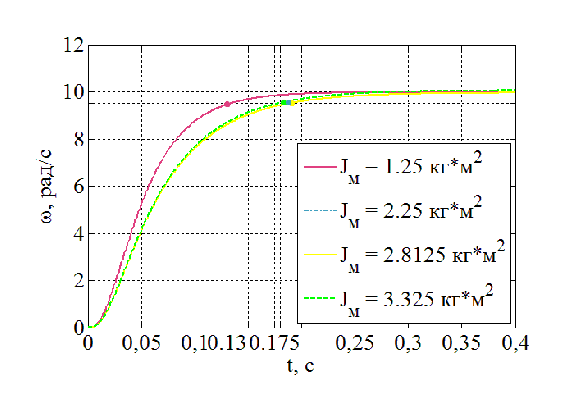
\includegraphics[width = \textwidth]{scheme/W2}
		\caption{Переходный процесс по угловой скорости}
	\end{subfigure}
	\hfill
	\begin{subfigure}[b]{0.48\textwidth}
		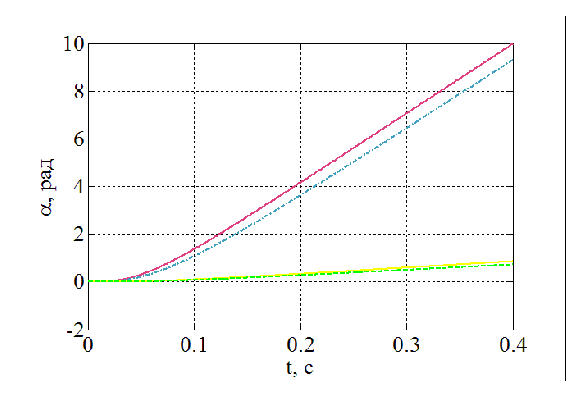
\includegraphics[width = \textwidth]{scheme/A2}
		\caption{Переходный процесс по углу поворота}
	\end{subfigure}
	\caption{Графики переходных процессов при различных значениях $J_M$}
	\label{UIwa2}
\end{figure}

\newpage
\section{Исследование передаточного отношения редуктора $i_p$ на вид переходных процессов}
Исследования проводились при величине момента сопротивления $M_{CM}=0$ и при $M_{CM}=46$. Графики переходных процессов изображены на рисунках \ref{UIwa00} и \ref{UIwa44} соответственно. Диапазон изменения передаточного отношения: $\pm 75\%$  от заданного значения. 
\begin{figure}[H]
	\centering
	\begin{subfigure}[b]{0.48\textwidth}
	    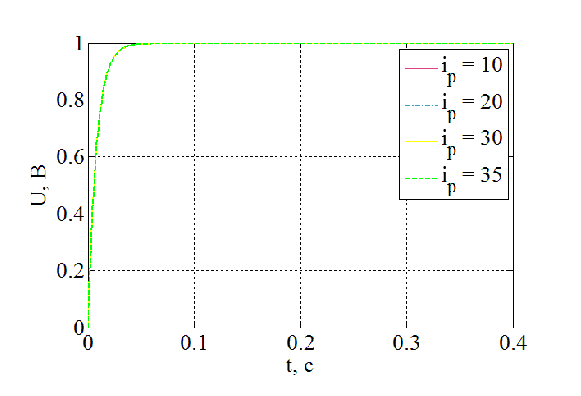
\includegraphics[width = \textwidth]{scheme/U3}
		\caption{Переходный процесс по напряжению}
	\end{subfigure}
	\hfill
	\begin{subfigure}[b]{0.48\textwidth}
		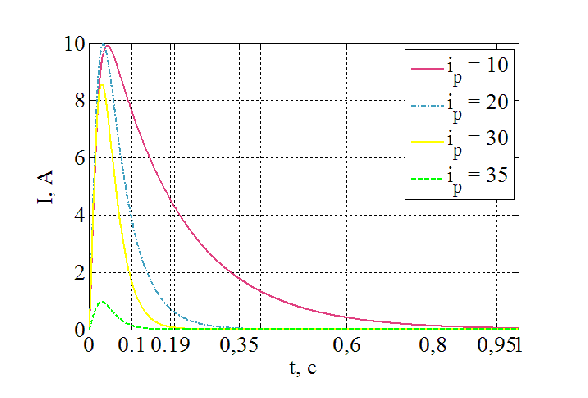
\includegraphics[width = \textwidth]{scheme/I3}
		\caption{Переходный процесс по току}
	\end{subfigure}
	\begin{subfigure}[b]{0.48\textwidth}
		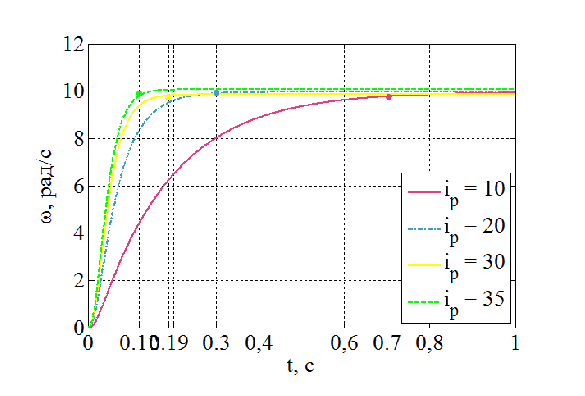
\includegraphics[width = \textwidth]{scheme/W3}
		\caption{Переходный процесс по угловой скорости}
	\end{subfigure}
	\hfill
	\begin{subfigure}[b]{0.48\textwidth}
		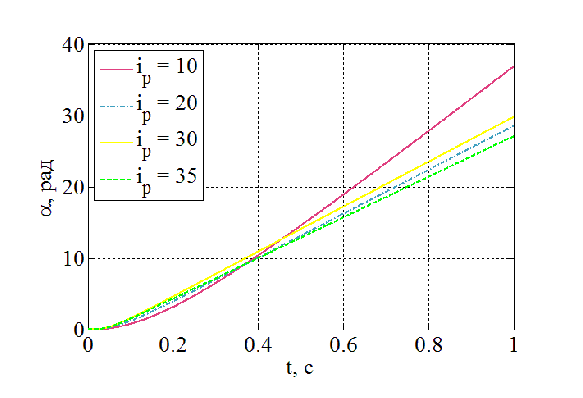
\includegraphics[width = \textwidth]{scheme/A3}
		\caption{Переходный процесс по углу поворота}
	\end{subfigure}
	\caption{Графики переходных процессов при различных значениях $i_p$ и $M_{CM}=0$}
	\label{UIwa00}
\end{figure}
\begin{figure}[H]
	\centering
	\begin{subfigure}[b]{0.48\textwidth}
	    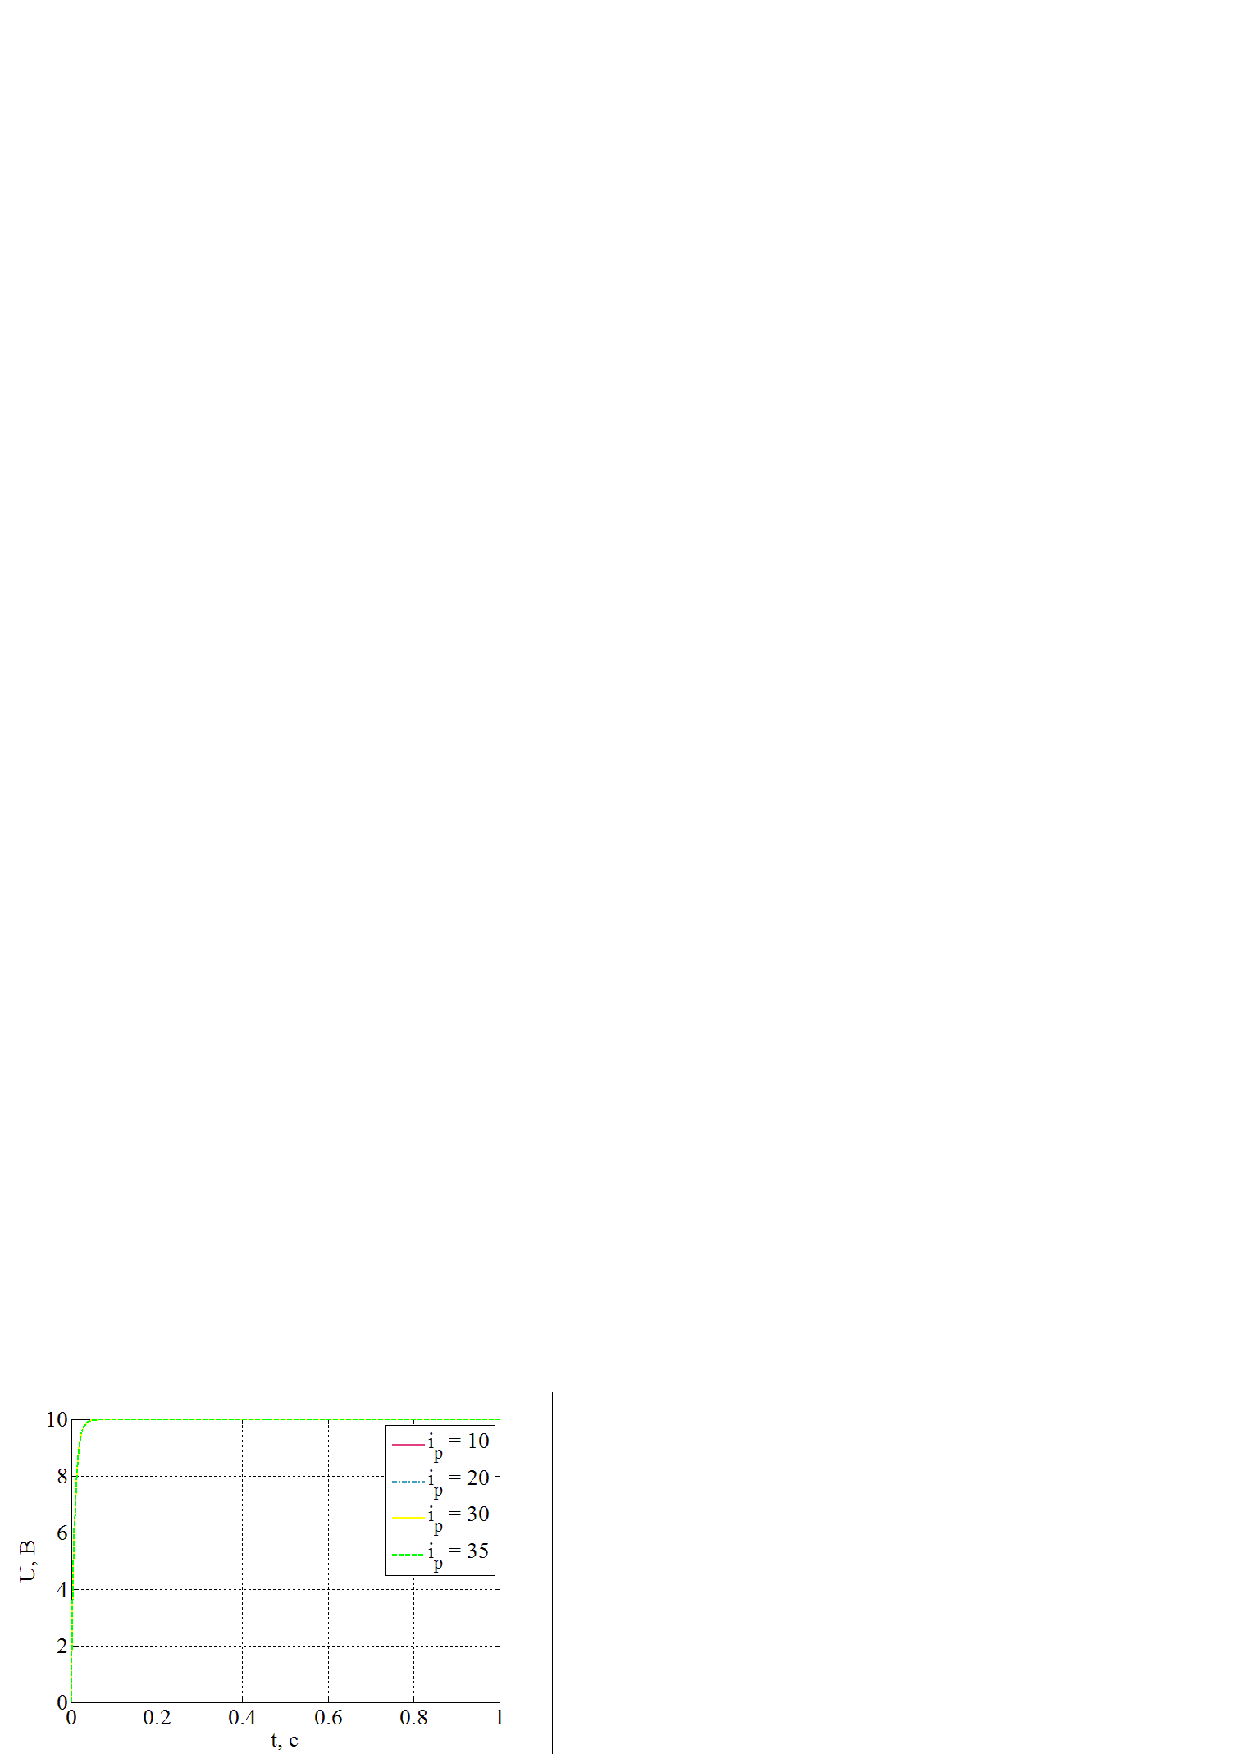
\includegraphics[width = \textwidth]{scheme/U4}
		\caption{Переходный процесс по напряжению}
	\end{subfigure}
	\hfill
	\begin{subfigure}[b]{0.48\textwidth}
		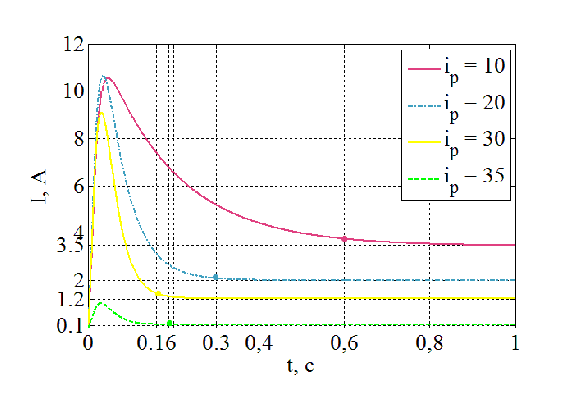
\includegraphics[width = \textwidth]{scheme/I4}
		\caption{Переходный процесс по току}
	\end{subfigure}
	\begin{subfigure}[b]{0.48\textwidth}
		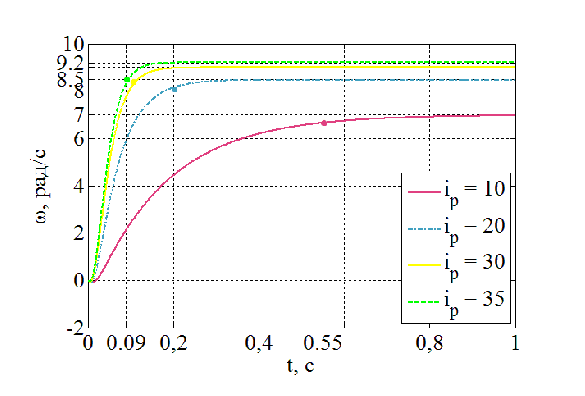
\includegraphics[width = \textwidth]{scheme/W4}
		\caption{Переходный процесс по угловой скорости}
	\end{subfigure}
	\hfill
	\begin{subfigure}[b]{0.48\textwidth}
		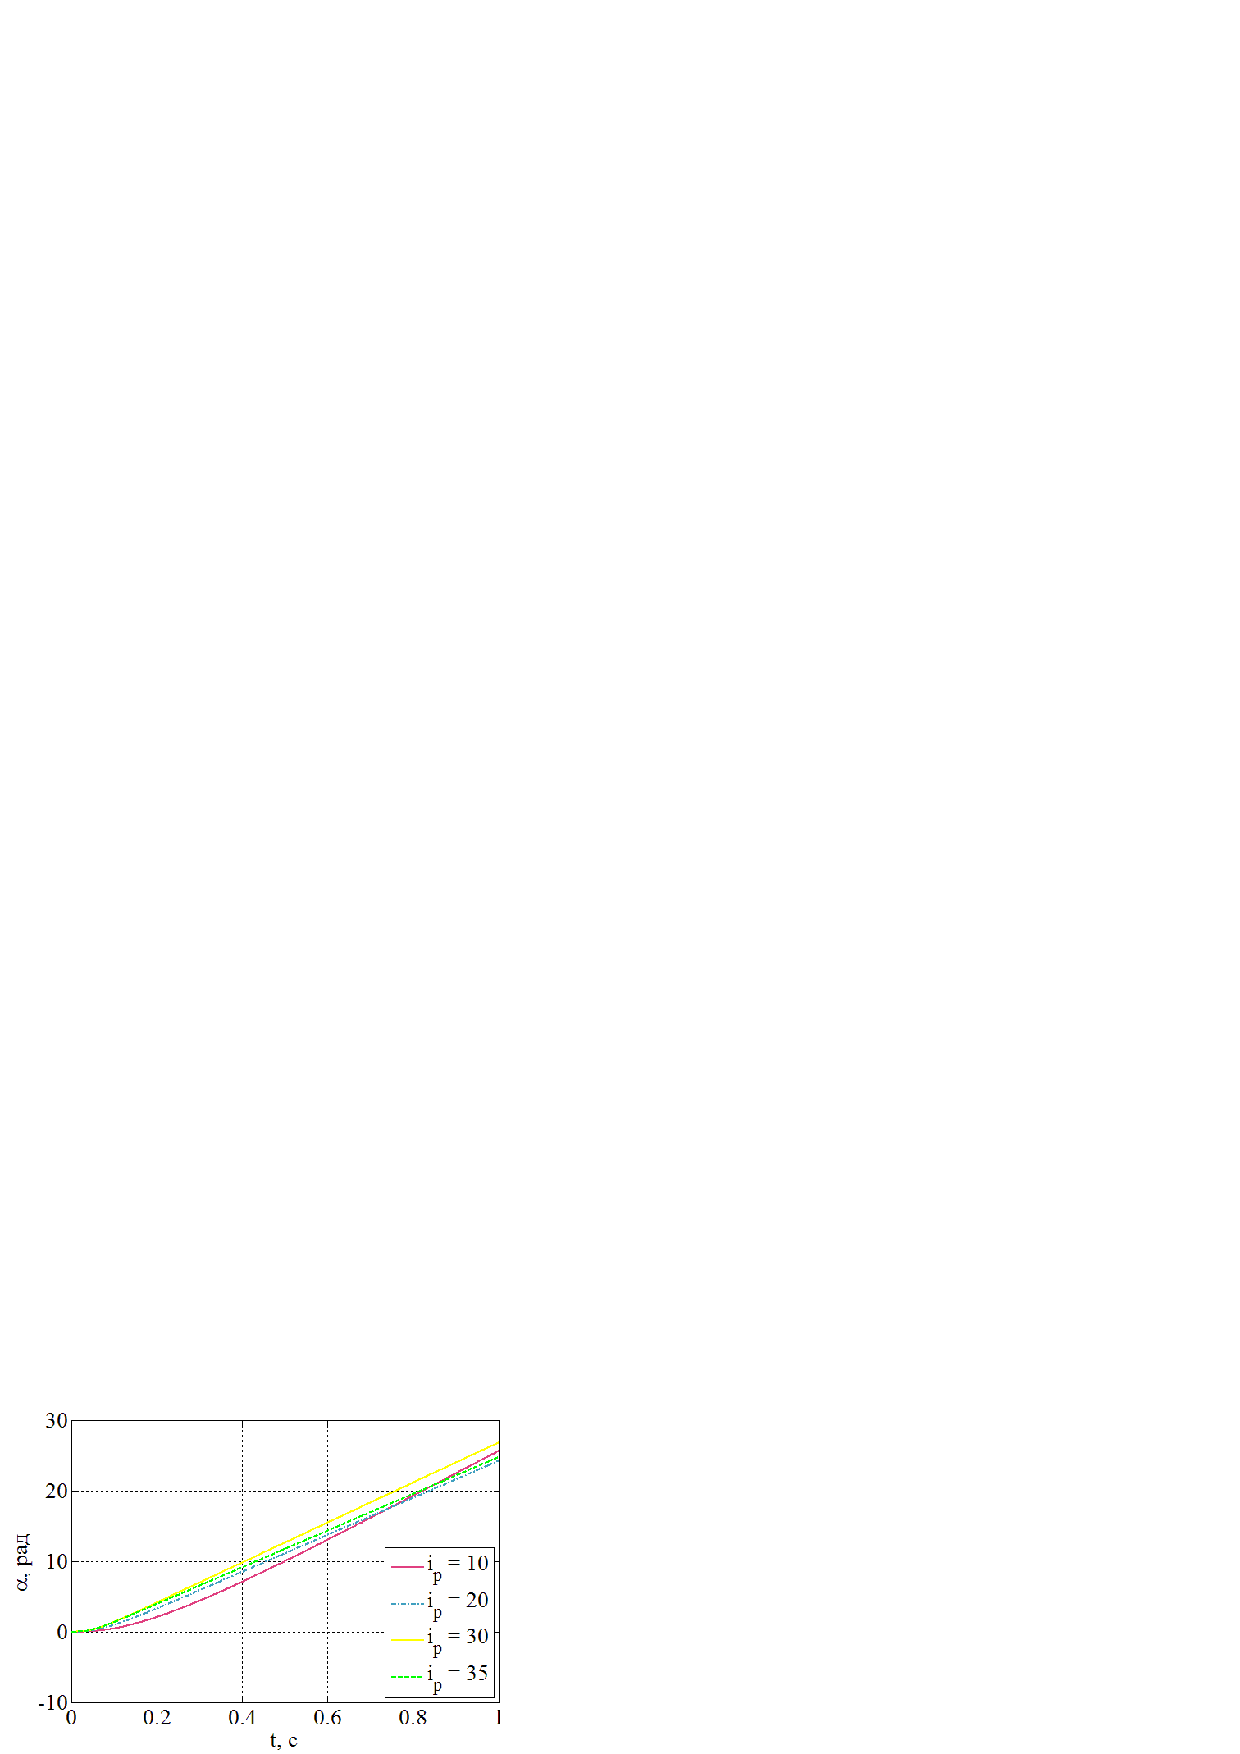
\includegraphics[width = \textwidth]{scheme/A4}
		\caption{Переходный процесс по углу поворота}
	\end{subfigure}
	\caption{Графики переходных процессов при различных значениях $i_p$ и $M_{CM}=46$}
	\label{UIwa44}
\end{figure}

\newpage
\section{Исследование влияния постоянных времени на вид переходных процессов}
Исследования проводились при значениях постоянных времени $T_\text{у} = \frac{8}{10} \text{мс} = 0,0008$c, $T_\text{я} = \frac{6}{10} \text{мс} = 0,001$c. Графики переходных процессов изображены на рисунке \ref{UIwa0056}.
\begin{figure}[H]
	\centering
	\begin{subfigure}[b]{0.48\textwidth}
	    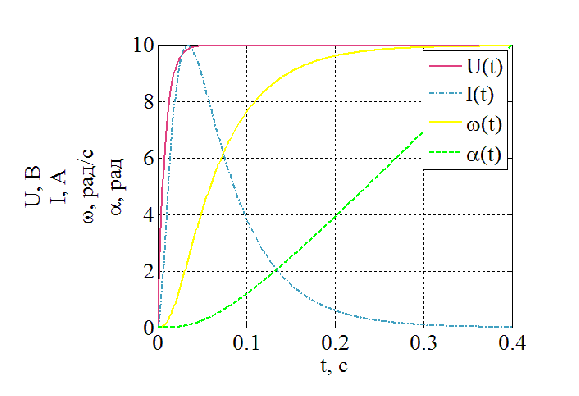
\includegraphics[width = \textwidth]{scheme/T0}
		\caption{$T_\text{у} = 0,008$c, $T_\text{я} = 0,01$c}
	\end{subfigure}
	\hfill
	\begin{subfigure}[b]{0.48\textwidth}
		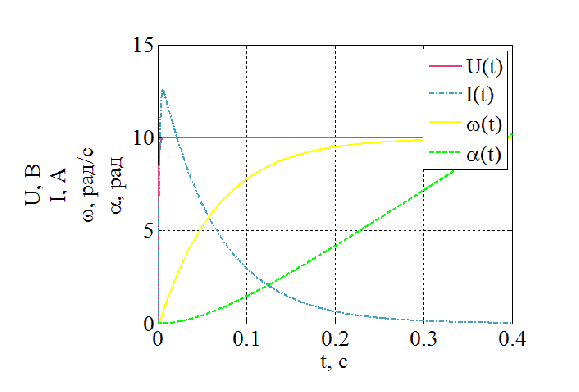
\includegraphics[width = \textwidth]{scheme/T1}
		\caption{$T_\text{у} = 0,0008$c, $T_\text{я} = 0,001$c}
	\end{subfigure}
	\caption{Графики переходных процессов при различных значениях постоянных времени}
	\label{UIwa0056}
\end{figure}

Из графиков (рисунок \ref{UIwa0056}) видно, что при уменьшении значений постоянных времени на порядок установившиеся значения тока и скорости, а также время переходного процесса этих величин не изменились, однако возросло максимальное значение тока.

\newpage
\section{Математическое моделирование упрощённой модели электромеханического объекта}	 
На основе структурной схемы, представленной на рисунке \ref{simpScheme}, составим схему моделирования ЭМО (рисунок \ref{cxema2}).
\begin{figure}[ht!]
	\centering
	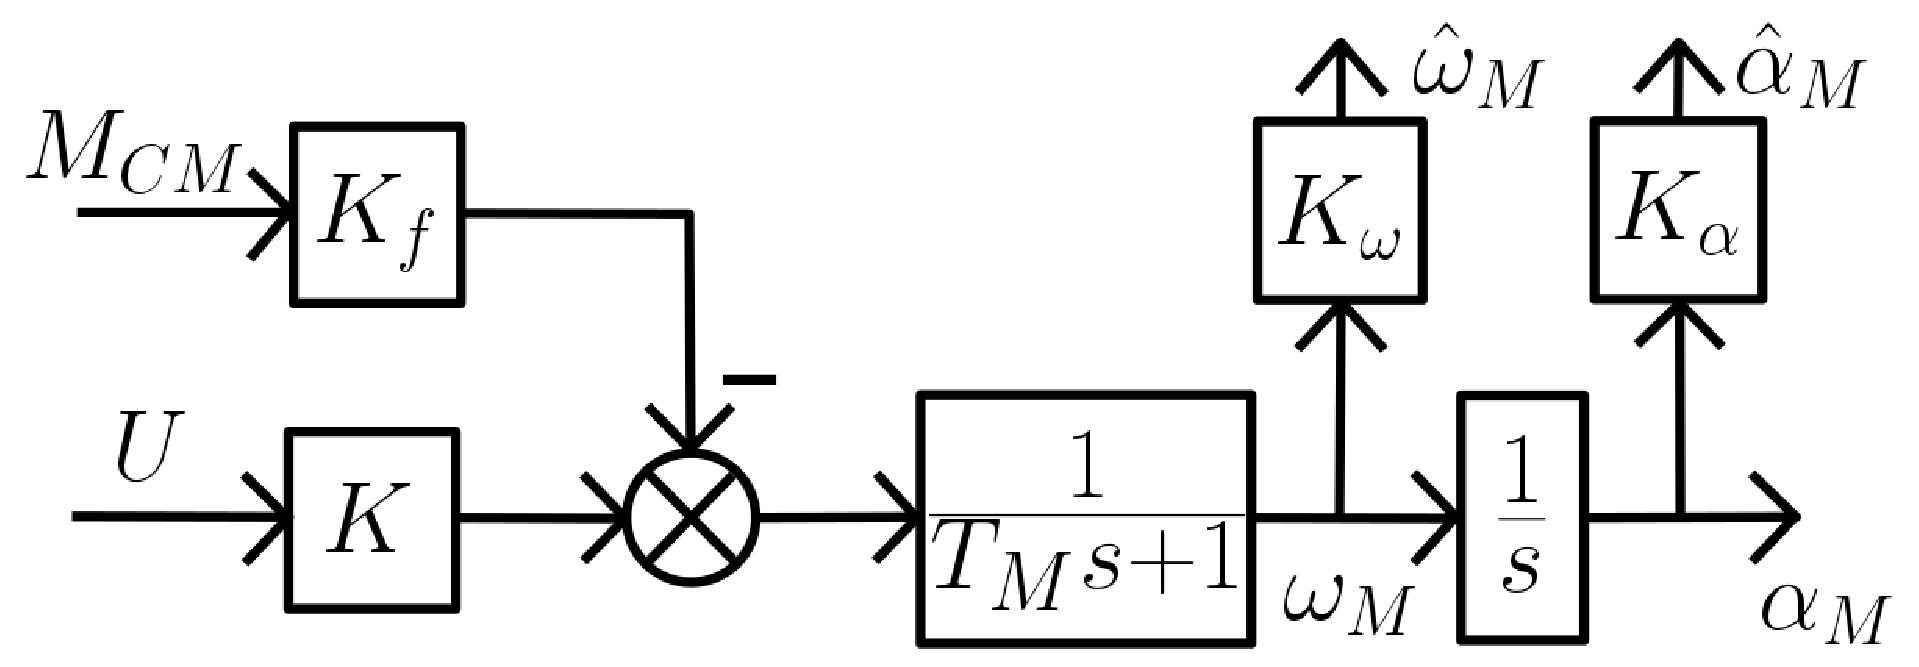
\includegraphics[width = \textwidth]{scheme/simpScheme}
	\caption{Структурная схема ЭМО}
	\label{simpScheme}
\end{figure}
\begin{figure}[ht!]
	\centering
 	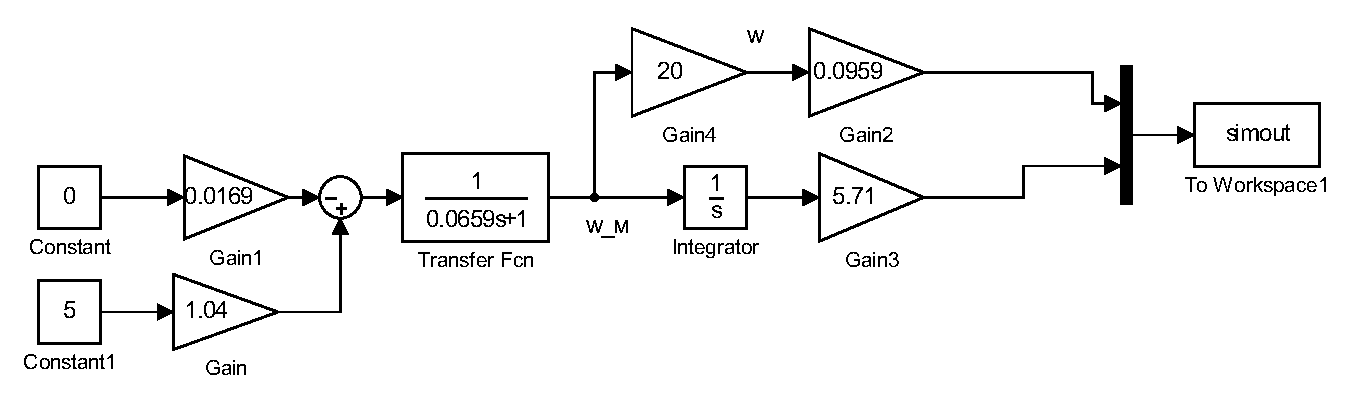
\includegraphics[width = \textwidth]{scheme/SRscheme}
	\caption{Схема моделирования ЭМО}
	\label{cxema2}
\end{figure}

Для того, чтобы проанализировать погрешности проведём сравнение графиков переходных процессов по угловой скорости полной и упрощённой модели ЭМО, а также полной модели при меньших значениях постоянных времени и упрощённой модели (рисунок \ref{sravnenie}). 
\begin{figure}[H]
	\centering
	\begin{subfigure}[b]{0.48\textwidth}
	    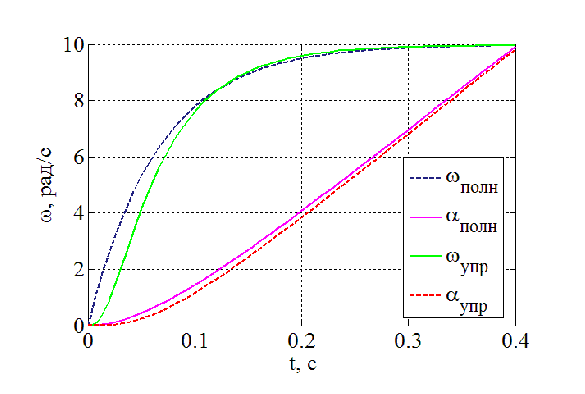
\includegraphics[width = \textwidth]{scheme/SR1}
		\caption{График сравнения переходных процессов полной модели ЭМО и упрощённой}
	\end{subfigure}
	\hfill
	\begin{subfigure}[b]{0.48\textwidth}
		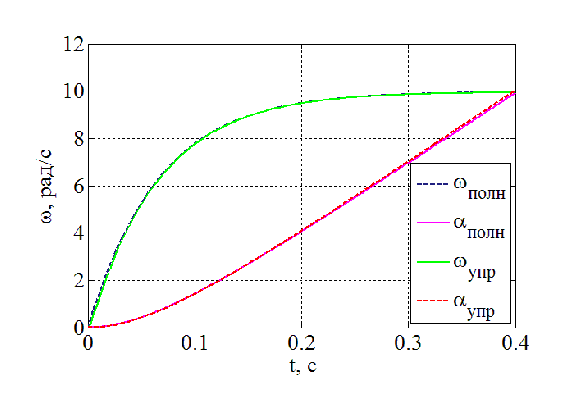
\includegraphics[width = \textwidth]{scheme/SR2}
		
		\caption{График сравнения переходных процессов полной модели ЭМО при меньших значениях постоянных времени и упрощённой модели}
	\end{subfigure}
	\caption{График сравнения переходных процессов полной и упрощённой модели ЭМО}
	\label{sravnenie}
\end{figure}

\newpage
\section{Вывод математических моделей вход-состояние-выход для полной и упрощенной схем моделирования ЭМО}
Полная модель ЭМО.\par
Для составления математической модели запишем формулы, характеризующие ЭМО, взятые из теории к данной лабораторной работе.
\begin{align}
	&&\begin{cases}
		T_\text{Я}\dot{I} + I = K_\text{Д}(U_\text{У} - K_E\omega)\\
		M_\text{Д} - M_C = J_\Sigma\dot{\omega}\\
		\dot{\alpha} = \omega\\
		T_\text{У}\dot{U_\text{У}} + U_\text{У} = K_\text{У}U
	\end{cases}
	\Rightarrow
	\begin{cases}
		\dot{I} = \displaystyle{- \frac{1}{T_\text{Я}}I + \frac{K_\text{Д}}{T_\text{Я}}U_\text{У} -\frac{K_E}{T_\text{Я}}}\omega \\
		\dot{\omega} = \displaystyle{\frac{K_m}{J_\Sigma}}I - \frac{1}{J_\Sigma}M_C\\
		\dot{\alpha} = \omega\\
		\dot{U_\text{У}} = -\displaystyle{\frac{1}{T_\text{У}}U_\text{У}} + \frac{K_\text{У}}{T_\text{У}}U
	\end{cases}
	,
	\label{ESETh}
\end{align}
где $M_\text{Д} = K_mI$.
	
Примем вектор состояния
$
	X =
	\begin{bmatrix}
		\alpha & \omega & I & U_\text{У}
	\end{bmatrix}^T
$
и вектор входных воздействий
$
	U =
	\begin{bmatrix}
		U & M_C
	\end{bmatrix}^T,
$
тогда исходя из (\ref{ESETh}) получим модель Вход-Состояние-Выход:
\begin{align}
	\begin{cases}
		\dot{X} = AX + BU\\
		y = CX
	\end{cases} \Rightarrow
	\begin{cases}
		\begin{bmatrix}
			\dot{\alpha}\\
			\dot{\omega}\\
			\dot{I}\\
			\dot{U_\text{У}}
		\end{bmatrix} =
		\begin{bmatrix}
			0 & 1 & 0 & 0\\
			0 & 0 & \displaystyle{\frac{K_m}{J_\Sigma}} & 0\\
			0 & -\displaystyle{\frac{K_E}{T_\text{Я}}} & -\displaystyle{\frac{1}{T_\text{Я}}} & \displaystyle{\frac{K_\text{Д}}{T_\text{Я}}}\\
			0 & 0 & 0 & -\displaystyle{\frac{1}{T_\text{У}}}
		\end{bmatrix}
		\begin{bmatrix}
			\alpha\\
			\omega\\
			I\\
			U_\text{У}
		\end{bmatrix}
		+
		\begin{bmatrix}
			0 & 0\\
			0 & -\displaystyle{\frac{1}{J_\Sigma}}\\
			0 & 0\\
			\displaystyle{\frac{K_\text{У}}{T_\text{У}}} & 0
		\end{bmatrix}
		\begin{bmatrix}
			U\\
			M_C
		\end{bmatrix}\\
		\alpha = 
		\begin{bmatrix}
			1 & 0 & 0 & 0
		\end{bmatrix}
		\begin{bmatrix}
			\alpha\\
			\omega\\
			I\\
			U_\text{У}
		\end{bmatrix}.
	\end{cases}
	\label{ESEFull}
\end{align}
	
Подставив рассчитанные ранее значения, получим следующие матрицы
\begin{align}
	&&A = 
	\begin{bmatrix}
		0 & 1 & 0 & 0\\
		0 & 0 & 31.95 & 0\\
		0 & -31 & -100 & 153\\
		0 & 0 & 0 & -125
	\end{bmatrix}, B =
	\begin{bmatrix}
		0 & 0\\
		0 & -103.09\\
		0 & 0\\
		812.5 & 0
	\end{bmatrix}
\end{align}

Упрощенная модель.\par
Для составления упрощённой модели ЭМО постоянные времени $T_\text{У}$ и $T_\text{Я}$ приравнивают к 0, так как их значение существенно меньше, чем значение механической постоянной времени $T_M$. Для получения упрощённой модели Вход-Состояние-Выход произведём соответствующие подстановки в уравнения для полной системы (\ref{ESETh}).
\begin{align}
	&&\begin{cases}
		\dot{\omega} = -\displaystyle{\frac{K_MK_\text{Д}K_E}{J_\Sigma}}\omega + \frac{K_MK_\text{Д}K_E}{J_\Sigma}U - \frac{1}{J_\Sigma}M_C\\
		\dot{\alpha} = \omega
	\end{cases},
\end{align}
и на основании полученной системы построим модель:
\begin{align}
	&&\begin{cases}
		\begin{bmatrix}
			\dot{\alpha}\\
			\dot{\omega}
		\end{bmatrix} =
		\begin{bmatrix}
			0 & 1\\
			0 & -\displaystyle{\frac{K_MK_\text{Д}K_E}{J_\Sigma}}
		\end{bmatrix}
		\begin{bmatrix}
			\alpha\\
			\omega
		\end{bmatrix} + 
		\begin{bmatrix}
			0 & 0\\
			\displaystyle{\frac{K_MK_\text{Д}K_E}{J_\Sigma}} & -\displaystyle{\frac{1}{J_\Sigma}}
		\end{bmatrix}
		\begin{bmatrix}
			U\\
			M_C
		\end{bmatrix}\\
		\alpha =
		\begin{bmatrix}
			1 & 0
		\end{bmatrix}
		\begin{bmatrix}
			\alpha\\
			\omega
		\end{bmatrix}
	\end{cases}.
\end{align}
	
Подставив значения, получим матрицы:
\begin{align}
	&&A =
	\begin{bmatrix}
		0 & 1\\
		0 & -15,15
	\end{bmatrix}, B = 
	\begin{bmatrix}
		0 & 0\\
		15,15 & -103.09
	\end{bmatrix}
\end{align}

\newpage
\begin{center}
	\section*{Вывод}
\end{center}
\par
В ходе лабораторной работы было проведено исследование математических моделей электромеханического объекта управления. Были выявлены изменения в переходных процессах системы путём изменения таких параметров как момент сопротивления, момент нагрузки, передаточное отношение редуктора.\par
Как видно из рисунка \ref{UIwa1} при увеличении момента сопротивления установившееся значение тока якоря увеличивается, а значение угловой скорости уменьшается. Время переходного процесса по току уменьшается с 0,325с до 0,25с, а по скорости остается практически постоянным и равным 0,19с.\par
При исследовании момента инерции нагрузки было показано, что его увеличение ведёт к возрастанию времени переходного процесса по угловой скорости и по току, в то время как установившееся значение этих двух параметров остается неизменным, что можно увидеть на графике, изображенном на рисунке \ref{UIwa2}.\par
Так же можно наблюдать, что в случае нулевого момента сопротивления при увеличении передаточного отношения редуктора максимальное значение тока и время переходного процесса уменьшаются. Установившиеся значения тока и угловой скорости при этом остаются постоянными.\par
В случае момента сопротивления равном половине максимального значения при увеличении $i_p$ не только уменьшается время переходного процесса по току и скорости, а также установившееся значение тока, но и увеличивается установившееся значение скорости.\par
Как можно заметить по результатам математического моделирования при постоянных времени много меньших по сравнению с механической постоянной времени переходной процесс по скорости и углу поворота ротора не имеет значительных изменений, поэтому ими можно пренебречь и перейти к упрощенной модели.

\end{document}
